\documentclass[11pt,a4paper]{article}

\usepackage[utf8]{inputenc}
\usepackage[T1]{fontenc}
\usepackage[spanish,es-tabla]{babel}
\usepackage{lmodern}
\usepackage{microtype}
\usepackage[a4paper,margin=2.5cm,headheight=14pt]{geometry}
\usepackage{setspace}
\onehalfspacing
\usepackage{graphicx}
\usepackage{float}
\usepackage{booktabs}
\usepackage{longtable}
\usepackage{array}
\usepackage{tabularx}
\usepackage{enumitem}
\usepackage{amsmath}
\usepackage{xcolor}
\usepackage{listings}
\usepackage{tikz}
\usetikzlibrary{arrows.meta,positioning,fit,backgrounds,calc,shapes.geometric}
\usepackage[most]{tcolorbox}
\usepackage{fancyhdr}
\usepackage{caption}
\usepackage{needspace}
\usepackage{hyperref}

\definecolor{epnblue}{RGB}{20,70,130}
\definecolor{epnteal}{RGB}{0,110,110}
\definecolor{codegray}{RGB}{245,246,248}
\definecolor{rulegray}{RGB}{210,214,220}

\hypersetup{
  colorlinks=true,
  linkcolor=epnblue,
  citecolor=epnteal,
  urlcolor=epnblue,
  pdftitle={Proyecto Integrador del Primer Parcial - Backend V1 NestJS},
  pdfauthor={Dennison Chalcán, Fernando Sandoval, Jerson Llumiquinga},
  pdfsubject={Desarrollo Software Seguro}
}

\pagestyle{fancy}
\fancyhf{}
\fancyhead[L]{\small Desarrollo Software Seguro}
\fancyhead[R]{\small Proyecto Integrador --- Backend V1}
\fancyfoot[C]{\thepage}
\renewcommand{\headrulewidth}{0.4pt}
\renewcommand{\footrulewidth}{0pt}

\setlength{\parskip}{0.45em}
\setlength{\parindent}{1.2em}
\setlength{\emergencystretch}{3em}

\newcommand{\code}[1]{\texttt{\detokenize{#1}}}
\newcommand{\term}[1]{\textit{#1}}

\lstset{
  basicstyle=\ttfamily\small,
  breaklines=true,
  columns=fullflexible,
  keepspaces=true,
  frame=single,
  rulecolor=\color{rulegray},
  backgroundcolor=\color{codegray},
  showstringspaces=false,
  keywordstyle=\color{epnblue}\bfseries,
  commentstyle=\color{epnteal},
  stringstyle=\color{orange!70!black},
  captionpos=b,
  xleftmargin=0.4cm,
  xrightmargin=0.4cm
}

\newtcolorbox{resultbox}[1][]{
  colback=epnblue!4,
  colframe=epnblue!55,
  boxrule=0.6pt,
  arc=2pt,
  left=6pt,
  right=6pt,
  top=4pt,
  bottom=4pt,
  fonttitle=\bfseries,
  title={#1}
}

\begin{document}

\begin{titlepage}
  \thispagestyle{empty}
  \centering
  \vspace*{1.2cm}

  {\large \textsc{Departamento de Ciencias de la Computación (DCCO)}}\\[0.4cm]
  {\large \textsc{Desarrollo Software Seguro}}\\[2.2cm]

  \rule{\textwidth}{1.2pt}\\[0.5cm]
  {\LARGE \bfseries Proyecto Integrador del Primer Parcial}\\[0.5cm]
  {\Large \bfseries Backend V1: autenticación JWT/RBAC en NestJS y\\[0.15cm]
  detección de esteganografía LSB en imágenes}\\[0.5cm]
  \rule{\textwidth}{1.2pt}\\[2.0cm]

  {\large \bfseries Integrantes}\\[0.4cm]
  \begin{tabular}{c}
    Dennison Chalcán\\
    Fernando Sandoval\\
    Jerson Llumiquinga
  \end{tabular}\\[2.4cm]

  {\large \bfseries Fecha de entrega}\\[0.3cm]
  {\large 04 de noviembre de 2026}\\[2.2cm]

  \vfill
  {\small Documento técnico del sistema implementado. Versión 2.0, adaptada a la
  implementación real en NestJS.}\\
  {\small Repositorio: \code{secure-chat-proyecto-DJF}}
\end{titlepage}

\pagenumbering{roman}
\tableofcontents
\clearpage
\listoffigures
\listoftables
\clearpage
\pagenumbering{arabic}

% ============================================================
\section{Resumen}
% ============================================================

El presente proyecto implementa \textbf{Backend V1}, la primera entrega del backend de
una aplicación de salas de chat seguras, compuesta por dos microservicios REST
independientes desarrollados con \textbf{NestJS}. El primero, \textbf{AUTH}
(\code{ms-auth-nestjs}), administra identidades, roles, asignaciones usuario--rol,
emisión y revocación de tokens JWT firmados con RSA (RS256), y autorización interna
entre servicios. El segundo, \textbf{STEGO} (\code{ms-stego-nestjs}), recibe imágenes
PNG y BMP, valida su estructura con \term{magic bytes}, ejecuta un detector de
esteganografía LSB basado en entropía, igualación de pares y chi-cuadrado, y
clasifica el archivo como limpio, no concluyente o sospechoso.

La solución aplica los principios \term{Secure by Design}, \term{Zero Trust} y
\term{Shift Left}: el rol efectivo se consulta en PostgreSQL en cada operación, el
token no se considera una verdad permanente, los archivos se validan antes de
procesarse y la comunicación entre servicios se autentica con una clave de servicio
de 256 bits mediante el encabezado \code{X-Service-Key}. La clave privada RSA y las
bases de datos no se exponen fuera de la red interna de Docker.

El sistema se ejecuta con Docker Compose en seis servicios autónomos, incluye
migraciones y datos semilla, documentación OpenAPI/Swagger, y una suite de pruebas
automatizadas. La ejecución local reportó \textbf{83/83 pruebas unitarias aprobadas}
(36 de AUTH y 47 de STEGO). La suite e2e de AUTH comprende \textbf{30 pruebas} contra
PostgreSQL real y se ejecuta con Docker en marcha.

\begin{resultbox}[Resultado verificable]
Al cierre de esta adaptación, \code{npm test} reportó \textbf{36/36 pruebas aprobadas}
en AUTH y \textbf{47/47} en STEGO. Los servicios quedan publicados únicamente en
loopback: AUTH en \code{http://localhost:3001} y STEGO en
\code{http://localhost:3002}.
\end{resultbox}

\begin{quote}
\textbf{Palabras clave:} microservicios; NestJS; JWT; RBAC; Argon2id; esteganografía;
desarrollo seguro.
\end{quote}

% ============================================================
\section{Introducción}
% ============================================================

\subsection{Problema y contexto}

Los sistemas que reciben archivos de usuarios enfrentan dos riesgos simultáneos.
Por un lado, deben garantizar que solo identidades autenticadas y autorizadas
ejecuten operaciones sensibles. Por otro, deben impedir que archivos malformados,
excesivos o manipulados provoquen denegación de servicio, ejecución de código o
fuga de información. Cuando la autorización se resuelve únicamente en el cliente,
o cuando el token se emite sin posibilidad de revocación, el control de acceso
deja de ser vigente.

El proyecto aborda este problema mediante una separación estricta de
responsabilidades: AUTH decide \emph{quién es} el usuario y \emph{qué puede hacer};
STEGO decide \emph{si el archivo es procesable} y aplica la autorización recibida
de AUTH antes de analizarlo. La separación permite razonar sobre límites de
confianza, auditar cada decisión y escalar o aislar cada servicio de forma
independiente, con su propia base de datos y su propio ciclo de migraciones.

\subsection{Objetivo general}

Implementar un backend seguro de dos microservicios REST en NestJS que integre
autenticación JWT con RBAC dinámico, comunicación autenticada entre servicios y
análisis de esteganografía LSB en imágenes, con controles de validación,
trazabilidad y pruebas reproducibles.

\subsection{Objetivos específicos}

\begin{itemize}[leftmargin=1.4em]
  \item Diseñar un modelo de identidad con usuarios, roles y relación muchos a muchos.
  \item Emitir y verificar JWT RS256, con revocación por \code{tokenVersion} y consulta del rol efectivo en cada operación.
  \item Proteger los endpoints de STEGO mediante autorización interna de AUTH y vínculo de propiedad del resultado.
  \item Validar imágenes por extensión, \term{magic bytes}, tamaño, dimensiones y decodificación antes del análisis.
  \item Detectar indicios de esteganografía LSB y clasificar el archivo con una política explícita.
  \item Documentar la arquitectura, el contrato OpenAPI, los riesgos y la evidencia de pruebas.
\end{itemize}

\subsection{Alcance y limitaciones}

La versión implementa el backend y su operación local con Docker Compose. No incluye
interfaz gráfica ni despliegue en nube. El detector es una herramienta de triage:
reduce falsos positivos frente a una simple suma de LSB, pero no demuestra
criptográficamente la ausencia de información oculta. Los formatos soportados son
PNG y BMP verificados por extensión y \term{magic bytes}; el contenido se normaliza
con \code{sharp} a sRGB sin canal alfa. Los archivos de más de 10 MiB, con más de
10000 píxeles por lado o con más de 40 megapíxeles se rechazan de forma segura.
STEGO no conserva el archivo original ni una copia física de cuarentena: la acción
\code{cuarentena} es una decisión lógica registrada en la base de datos.

% ============================================================
\section{Arquitectura de la solución}
% ============================================================

\subsection{Vista de componentes}

La Tabla~\ref{tab:servicios} resume los servicios y su responsabilidad. AUTH es el
único componente que conoce contraseñas, roles y la clave privada. STEGO nunca recibe
la contraseña ni la clave privada; solo verifica la firma del JWT con la clave
pública montada en modo de solo lectura y solicita a AUTH la decisión de autorización
para la acción concreta.

\begin{table}[htbp]
  \centering
  \small
  \caption{Servicios de Backend V1.}
  \label{tab:servicios}
  \begin{tabularx}{\textwidth}{@{}l l X@{}}
    \toprule
    \textbf{Servicio} & \textbf{Puerto} & \textbf{Responsabilidad} \\
    \midrule
    \code{auth-db} & Interno & PostgreSQL 18 Alpine para identidades, roles, asignaciones y \code{token_version}. \\
    \code{auth-migrate} & --- & Ejecuta las migraciones de AUTH una sola vez y termina. \\
    AUTH & \code{3001} & Identidades, roles, asignaciones N:M, JWT RS256, RBAC dinámico y autorización interna con \code{X-Service-Key}. \\
    \code{stego-db} & Interno & PostgreSQL 18 Alpine para los resultados de análisis. \\
    \code{stego-migrate} & --- & Ejecuta las migraciones de STEGO una sola vez y termina. \\
    STEGO & \code{3002} & Validación de imágenes, detector LSB, clasificación y persistencia de resultados. \\
    \bottomrule
  \end{tabularx}
\end{table}

\begin{figure}[htbp]
  \centering
  \resizebox{\textwidth}{!}{%
  \begin{tikzpicture}[
    font=\small,
    box/.style={draw, rounded corners, fill=epnblue!6, minimum width=3.2cm, minimum height=1.15cm, align=center, thick},
    svc/.style={draw, rounded corners, fill=orange!8, minimum width=3.4cm, minimum height=1.2cm, align=center, thick},
    db/.style={draw, cylinder, shape border rotate=90, aspect=0.28, fill=epnteal!8, minimum width=3.1cm, minimum height=1.7cm, align=center, thick},
    job/.style={draw, dashed, rounded corners, fill=gray!8, minimum width=3.2cm, minimum height=0.9cm, align=center, thick},
    arr/.style={-{Latex[length=2.2mm]}, thick},
    dasharr/.style={-{Latex[length=2.2mm]}, thick, dashed},
    lbl/.style={font=\scriptsize, align=center, fill=white, inner sep=1pt}
  ]
    \node[box] (client) at (0,0) {Cliente REST\\\scriptsize Swagger / Postman};
    \node[job] (amig) at (6.6,4.6) {\code{auth-migrate}\\\scriptsize ejecución única};
    \node[job] (smig) at (6.6,-4.6) {\code{stego-migrate}\\\scriptsize ejecución única};
    \node[svc] (auth) at (6.6,2.2) {AUTH\\\scriptsize :3001};
    \node[svc] (stego) at (6.6,-2.2) {STEGO\\\scriptsize :3002};
    \node[db] (authdb) at (13.2,2.2) {\code{auth-db}\\\scriptsize PostgreSQL 18};
    \node[db] (stegodb) at (13.2,-2.2) {\code{stego-db}\\\scriptsize PostgreSQL 18};

    \draw[arr] (client.east) -- node[lbl, above, sloped] {1. login / JWT} (auth.west);
    \draw[arr] (client.east) to[bend right=12] node[lbl, below, sloped] {2. Bearer + imagen} (stego.west);
    \draw[arr] (stego.north) to[bend left=18] node[lbl, left=2pt] {3. \code{X-Service-Key}} (auth.south);
    \draw[dasharr] (auth.south east) to[bend left=18] node[lbl, right=2pt] {4. \code{public.pem} :ro} (stego.north east);
    \draw[arr] (auth.east) -- node[lbl, above] {SQL} (authdb.west);
    \draw[arr] (stego.east) -- node[lbl, above] {SQL} (stegodb.west);
    \draw[dasharr] (amig.south) -- (authdb.north);
    \draw[dasharr] (smig.north) -- (stegodb.south);

    \begin{scope}[on background layer]
      \node[draw, dashed, red!60, rounded corners, fit=(client), inner sep=8pt,
            label={[red!70]above:Zona no confiable}] {};
      \node[draw, dashed, epnteal!70, rounded corners, fit=(auth)(stego)(authdb)(stegodb)(amig)(smig), inner sep=12pt,
            label={[epnteal!80]above:Backend V1 --- red interna Docker \code{backend}}] {};
    \end{scope}
  \end{tikzpicture}}
  \caption{Arquitectura de componentes y límites de confianza. Las bases de datos no publican puertos al host; las APIs se publican solo en \code{127.0.0.1}.}
  \label{fig:arquitectura}
\end{figure}

\subsection{Flujo de una solicitud de análisis}

\begin{enumerate}[leftmargin=1.5em]
  \item El usuario se autentica en \code{POST /api/auth/login}. AUTH verifica la contraseña con Argon2id y emite un JWT RS256 de corta duración; los roles se devuelven en el cuerpo de la respuesta, no dentro del token.
  \item El cliente envía el JWT y la imagen a \code{POST /api/steganography/analyze}.
  \item STEGO verifica firma, algoritmo, emisor, audiencia, expiración y tipo \code{access}; la clave pública se monta desde \code{public.pem} en modo de solo lectura.
  \item STEGO llama a AUTH mediante \code{POST /internal/authorization/check}, enviando el encabezado \code{X-Service-Key} y el JWT del usuario en el cuerpo como \code{subject_token}.
  \item AUTH compara la clave de servicio en tiempo constante, verifica el JWT, resuelve el rol efectivo en PostgreSQL y comprueba que la acción esté permitida.
  \item Si AUTH no responde en el tiempo configurado (\code{AUTH_TIMEOUT_MS}, 3000 ms), o la decisión es incoherente, STEGO devuelve \code{503} y \textbf{no procesa el archivo}.
  \item Si la autorización es válida, STEGO valida el archivo, ejecuta el detector, persiste el resultado y responde con la clasificación.
\end{enumerate}

\subsection{Límites de confianza}

\begin{table}[htbp]
  \centering
  \small
  \caption{Controles en los límites de confianza.}
  \label{tab:limites}
  \begin{tabularx}{\textwidth}{@{}p{3.3cm} X X@{}}
    \toprule
    \textbf{Límite} & \textbf{Amenaza principal} & \textbf{Control implementado} \\
    \midrule
    Cliente $\rightarrow$ AUTH & Credenciales débiles o fuerza bruta & Argon2id, validación con DTO y Zod, \term{rate limit} y mensajes genéricos. \\
    Cliente $\rightarrow$ STEGO & Archivo malicioso o token robado & Verificación RS256, autorización vigente en AUTH, límites de tamaño y validación por \term{magic bytes}. \\
    STEGO $\rightarrow$ AUTH & Suplantación entre servicios & Red interna, \code{X-Service-Key} de 256 bits, comparación en tiempo constante y cuerpo con \code{subject_token}. \\
    AUTH $\rightarrow$ \code{auth-db} & Acceso directo a datos & Base sin puerto público, consultas parametrizadas por TypeORM y credenciales por variables de entorno. \\
    STEGO $\rightarrow$ \code{stego-db} & Lectura de resultados ajenos & Base aislada, sin tablas de AUTH, verificación de propiedad y acción \code{read.any} en AUTH. \\
    Claves RSA & Fuga de la clave privada & \code{private.pem} solo en AUTH y en un volumen de solo lectura; STEGO monta únicamente \code{public.pem}. \\
    \bottomrule
  \end{tabularx}
\end{table}

\subsection{Tecnologías}

\begin{table}[htbp]
  \centering
  \small
  \caption{Tecnologías y propósito.}
  \label{tab:tecnologias}
  \begin{tabularx}{\textwidth}{@{}l X@{}}
    \toprule
    \textbf{Tecnología} & \textbf{Uso en el proyecto} \\
    \midrule
    Node.js 24 (Alpine) y NestJS 12 & Runtime y framework de ambos servicios. \\
    TypeORM & Entidades, migraciones versionadas y consultas parametrizadas. \\
    PostgreSQL 18 Alpine & Persistencia relacional separada para AUTH y STEGO. \\
    \code{@nestjs/jwt} + \code{passport-jwt} & Firma y verificación JWT RS256; sin algoritmos simétricos. \\
    \code{argon2} & Hash de contraseñas con Argon2id. \\
    \code{sharp} & Decodificación de imágenes, normalización a sRGB y análisis LSB. \\
    \code{multer} + \code{FileInterceptor} & Recepción en memoria de un único archivo multipart. \\
    \code{class-validator} + \code{zod} & Validación de DTO y del entorno de ejecución. \\
    \code{@nestjs/throttler} & Límite global y límites específicos en login y escrituras. \\
    \code{@nestjs/swagger} & Contrato OpenAPI y Swagger UI en \code{/docs}. \\
    Vitest y Supertest & Pruebas unitarias y e2e. \\
    Docker Compose & Orquestación de seis servicios, red, volúmenes y healthchecks. \\
    \bottomrule
  \end{tabularx}
\end{table}

% ============================================================
\section{Modelo de identidad y datos}
% ============================================================

\subsection{Modelo entidad--relación}

El modelo separa identidad, catálogo de roles y asignaciones. La tabla intermedia
\code{user_roles} tiene un índice único \code{(user_id, role_id)} y claves
foráneas con \code{ON DELETE CASCADE}; esto impide duplicados a nivel de base de
datos y elimina asignaciones huérfanas. La revocación de sesiones no usa una tabla
de tokens: se implementa con la columna \code{token_version} en \code{users}.

\begin{figure}[htbp]
  \centering
  \resizebox{\textwidth}{!}{%
  \begin{tikzpicture}[
    entity/.style={draw, rounded corners, fill=epnblue!5, align=left, text width=5.1cm, inner sep=6pt, font=\footnotesize\ttfamily, thick},
    arr/.style={thick},
    lab/.style={font=\scriptsize\bfseries}
  ]
    \node[entity] (users) at (0,0) {\textbf{users}\\[2pt]
      \underline{id} UUID PK\\
      cedula VARCHAR(10) UK\\
      nombres VARCHAR(100)\\
      apellidos VARCHAR(100)\\
      fecha\_nacimiento DATE\\
      username VARCHAR(50) UK\\
      email VARCHAR(150) UK\\
      telefono VARCHAR(10) UK\\
      password VARCHAR(255)\\
      status BOOLEAN\\
      token\_version INT\\
      version INT\\
      created\_at, updated\_at\\
      deleted\_at TIMESTAMP NULL};
    \node[entity] (roles) at (10.6,0) {\textbf{roles}\\[2pt]
      \underline{id} UUID PK\\
      rol VARCHAR(50) UK\\
      status BOOLEAN\\
      version INT\\
      created\_at, updated\_at\\
      deleted\_at TIMESTAMP NULL};
    \node[entity] (ur) at (5.3,-6.1) {\textbf{user\_roles}\\[2pt]
      \underline{id} UUID PK\\
      user\_id UUID FK\\
      role\_id UUID FK\\
      assigned\_at TIMESTAMP\\
      status BOOLEAN\\
      version INT\\
      created\_at, updated\_at\\
      UNIQUE(user\_id, role\_id)};

    \draw[arr] (users.south) -- node[lab, left]{1} (ur.north west);
    \draw[arr] (roles.south) -- node[lab, right]{1} (ur.north east);
    \node[lab] at (2.75,-3.55) {N};
    \node[lab] at (7.75,-3.55) {N};
    \node[font=\scriptsize, anchor=north] at (5.3,-8.5) {Cada usuario puede tener varios roles y cada rol varios usuarios.};
  \end{tikzpicture}}
  \caption{Modelo entidad--relación de AUTH.}
  \label{fig:er}
\end{figure}

\subsection{Esquema principal}

\begin{lstlisting}[caption={Extracto de \code{ms-auth-nestjs/src/database/migrations/1700000000000-InitialSchema.ts}.},label={lst:sql}]
CREATE TABLE IF NOT EXISTS "users" (
  "id" uuid NOT NULL DEFAULT gen_random_uuid(),
  "cedula" varchar(10) NOT NULL,
  "nombres" varchar(100) NOT NULL,
  "apellidos" varchar(100) NOT NULL,
  "fecha_nacimiento" date NOT NULL,
  "username" varchar(50) NOT NULL,
  "email" varchar(150) NOT NULL,
  "telefono" varchar(10) NOT NULL,
  "password" varchar(255) NOT NULL,
  "status" boolean NOT NULL DEFAULT true,
  "token_version" integer NOT NULL DEFAULT 0,
  "version" integer NOT NULL DEFAULT 1,
  "created_at" TIMESTAMP NOT NULL DEFAULT now(),
  "updated_at" TIMESTAMP NOT NULL DEFAULT now(),
  "deleted_at" TIMESTAMP NULL,
  CONSTRAINT "PK_users" PRIMARY KEY ("id")
);

CREATE TABLE IF NOT EXISTS "roles" (
  "id" uuid NOT NULL DEFAULT gen_random_uuid(),
  "rol" varchar(50) NOT NULL,
  "status" boolean NOT NULL DEFAULT true,
  "version" integer NOT NULL DEFAULT 1,
  "created_at" TIMESTAMP NOT NULL DEFAULT now(),
  "updated_at" TIMESTAMP NOT NULL DEFAULT now(),
  "deleted_at" TIMESTAMP NULL,
  CONSTRAINT "PK_roles" PRIMARY KEY ("id")
);

CREATE TABLE IF NOT EXISTS "user_roles" (
  "id" uuid NOT NULL DEFAULT gen_random_uuid(),
  "user_id" uuid NOT NULL,
  "role_id" uuid NOT NULL,
  "assigned_at" TIMESTAMP NOT NULL DEFAULT now(),
  "status" boolean NOT NULL DEFAULT true,
  "version" integer NOT NULL DEFAULT 1,
  "created_at" TIMESTAMP NOT NULL DEFAULT now(),
  "updated_at" TIMESTAMP NOT NULL DEFAULT now(),
  CONSTRAINT "PK_user_roles" PRIMARY KEY ("id"),
  CONSTRAINT "FK_user_roles_user" FOREIGN KEY ("user_id")
    REFERENCES "users"("id") ON DELETE CASCADE,
  CONSTRAINT "FK_user_roles_role" FOREIGN KEY ("role_id")
    REFERENCES "roles"("id") ON DELETE CASCADE
);
\end{lstlisting}

\subsection{Datos semilla}

La migración y el \term{seed} son idempotentes. La contraseña de los usuarios de
demostración es \code{ClaveSegura2026!} únicamente para desarrollo local; en un
entorno real debe reemplazarse. El archivo \code{.env} real está ignorado y no debe
distribuirse.

\begin{table}[htbp]
  \centering
  \small
  \caption{Usuarios semilla y roles.}
  \label{tab:seed}
  \begin{tabular}{@{}l l l@{}}
    \toprule
    \textbf{Usuario} & \textbf{Roles} & \textbf{Propósito} \\
    \midrule
    \code{jperez}   & \code{ADMIN}              & Administración completa. \\
    \code{cvega}    & \code{USER}, \code{ANALYST} & Demuestra múltiples roles simultáneos. \\
    \code{amendoza} & \code{ANALYST}            & Análisis y consulta de resultados propios. \\
    \code{mgomez}   & \code{USER}               & Sujeto sin permiso de análisis. \\
    \code{lcastro}  & \code{USER}               & Sujeto sin permiso de análisis. \\
    \bottomrule
  \end{tabular}
\end{table}

\subsection{Persistencia de STEGO}

STEGO usa su propia base de datos PostgreSQL, separada de AUTH. Guarda cada análisis
en la tabla \code{stego_analysis} con los campos \code{id}, \code{user_id},
\code{filename}, \code{sha256}, \code{technique}, \code{status}, \code{indicators}
(JSONB), \code{action}, \code{limitations} y \code{created_at}. El SHA-256 se calcula
sobre los bytes originales recibidos, antes de cualquier decodificación. La imagen no
se escribe en disco: se procesa en memoria y se descarta al terminar la solicitud. La
consulta \code{GET} verifica que el sujeto sea propietario del resultado o tenga
permiso \code{read.any} mediante AUTH.

% ============================================================
\section{Microservicio AUTH}
% ============================================================

\subsection{Contraseñas e identidad}

Las contraseñas se almacenan exclusivamente como hash \textbf{Argon2id} con
\code{memoryCost: 19456} KiB, \code{timeCost: 2} y \code{parallelism: 1}. El login
crea un hash ficticio al iniciar el módulo y compara siempre contra un hash válido,
incluso cuando el usuario no existe, para reducir diferencias de tiempo. Las
respuestas de error no revelan si el usuario existe: toda falla de credenciales
responde con \code{Credenciales inválidas}. El campo \code{password} está excluido de
la serialización y no se selecciona por defecto en las consultas.

\subsection{JWT RS256}

AUTH y STEGO comparten un par RSA de 2048 bits generado fuera de la imagen. La clave
privada reside en \code{ms-auth-nestjs/keys/private.pem} y solo se monta en AUTH; la
clave pública se monta en STEGO con la opción \code{:ro}. No existe endpoint JWKS: la
distribución de la clave pública es por volumen de solo lectura. El token se firma
con \code{RS256} y se verifica con algoritmo permitido explícito, emisor, audiencia,
expiración y tipo \code{access}; no se acepta \code{none} ni algoritmos simétricos.

\begin{table}[htbp]
  \centering
  \small
  \caption{Claims del JWT.}
  \label{tab:claims}
  \begin{tabularx}{\textwidth}{@{}l l X@{}}
    \toprule
    \textbf{Claim} & \textbf{Tipo} & \textbf{Uso} \\
    \midrule
    \code{sub} & UUID & Identificador del usuario. \\
    \code{username} & string & Nombre de usuario para trazabilidad. \\
    \code{tokenVersion} & numérico & Versión de sesión para revocación inmediata. \\
    \code{typ} & string & Debe ser \code{access}; otros valores se rechazan. \\
    \code{iss} & string & Emisor esperado: \code{ms-auth}. \\
    \code{aud} & string & Audiencia esperada: \code{secure-chat-api}. \\
    \code{iat}, \code{exp} & numérico & Emisión y expiración (900 segundos por defecto). \\
    \bottomrule
  \end{tabularx}
\end{table}

Los roles \textbf{no} se incluyen en el JWT. El login devuelve
\code{accessToken}, \code{tokenType} y un objeto \code{user} con el nombre de usuario
y los roles vigentes leídos de PostgreSQL.

\subsection{RBAC vigente}

Los roles se consultan en la base de datos en cada solicitud, por lo que un cambio de
rol surte efecto de inmediato aunque el token siga vigente criptográficamente. Si a
un usuario se le retira un rol, su token anterior deja de servir para esa acción. Lo
mismo ocurre con asignaciones desactivadas: el \term{guard} de roles deniega por
defecto toda ruta privada que no declare roles o la marca de acceso autenticado.

\begin{table}[htbp]
  \centering
  \small
  \caption{Matriz de roles y permisos.}
  \label{tab:rbac}
  \begin{tabularx}{\textwidth}{@{}>{\raggedright\arraybackslash}p{8.4cm} c c c@{}}
    \toprule
    \textbf{Acción} & \textbf{ADMIN} & \textbf{ANALYST} & \textbf{USER} \\
    \midrule
    Gestionar usuarios, roles y asignaciones & Sí & No & No \\
    \code{steganography.analyze} & Sí & Sí & No \\
    \code{steganography.results.read.own} & Sí & Sí & Sí \\
    \code{steganography.results.read.any} & Sí & No & No \\
    Consultar perfil propio (\code{/api/auth/profile}) & Sí & Sí & Sí \\
    \bottomrule
  \end{tabularx}
\end{table}

\subsection{Autorización interna entre servicios}

STEGO no puede confiar únicamente en el JWT para decidir una acción, porque el
usuario pudo perder el rol o cerrar sesión después de la emisión. Por eso consulta a
AUTH. La solicitud interna incluye el encabezado \code{X-Service-Key}, cuyo valor es
una clave compartida de 256 bits (\code{INTERNAL_API_KEY}) comparada en tiempo
constante, y un cuerpo con \code{subject_token}, \code{action} y
\code{resource_id} opcional. AUTH verifica el JWT, carga el usuario y sus roles
activos desde PostgreSQL, comprueba \code{tokenVersion} y responde con una decisión
explícita.

\begin{lstlisting}[caption={Cuerpo de la consulta interna de autorización.}]
POST /internal/authorization/check
X-Service-Key: <INTERNAL_API_KEY>

{
  "subject_token": "<JWT del usuario>",
  "action": "steganography.analyze",
  "resource_id": null
}
\end{lstlisting}

AUTH distingue los motivos \code{subject_not_active}, \code{token_revoked},
\code{unsupported_action} e \code{insufficient_permissions}. Si falla la
persistencia después de validar el token, responde \code{allowed: false} con motivo
\code{authorization_unavailable}. STEGO aplica \term{fail closed}: si AUTH no
responde, devuelve \code{503} y no procesa ni persiste el archivo.

\subsection{Revocación y cierre de sesión}

\code{POST /api/auth/logout} incrementa la columna \code{users.token_version}. El JWT
incluye el valor de \code{tokenVersion} al momento de la emisión; en cada verificación
se compara con el valor actual de la base. Una diferencia produce \code{401} con el
mensaje \code{La sesión ha expirado}. Esta revocación sobrevive a reinicios del
servicio porque reside en PostgreSQL y no en memoria. No existe una tabla de tokens
revocados ni un mecanismo de refresh token.

\subsection{Endpoints de AUTH}

\begin{small}
\begin{longtable}{@{}p{1.25cm}>{\raggedright\arraybackslash}p{7.0cm}>{\raggedright\arraybackslash}p{3.0cm}>{\raggedright\arraybackslash}p{2.9cm}@{}}
  \caption{Endpoints de AUTH.}\label{tab:endpoints-auth}\\
  \toprule
  \textbf{Método} & \textbf{Ruta} & \textbf{Acceso} & \textbf{Respuesta} \\
  \midrule
  \endfirsthead
  \toprule
  \textbf{Método} & \textbf{Ruta} & \textbf{Acceso} & \textbf{Respuesta} \\
  \midrule
  \endhead
  \bottomrule
  \endfoot
  POST & \code{/api/auth/login} & Público, rate limit 5/min & \code{200} token / \code{401} \\
  POST & \code{/api/auth/logout} & Autenticado & \code{204} \\
  GET  & \code{/api/auth/profile} & Autenticado & \code{200} perfil \\
  GET  & \code{/api/auth/me} & Autenticado (alias) & \code{200} perfil \\
  GET  & \code{/api/users} & ADMIN & \code{200} lista paginada \\
  POST & \code{/api/users} & ADMIN & \code{201} / \code{409} \\
  GET  & \code{/api/users/cedula/:cedula} & ADMIN & \code{200} / \code{404} \\
  GET  & \code{/api/users/:id} & ADMIN & \code{200} / \code{404} \\
  PATCH & \code{/api/users/:id} & ADMIN & \code{200} \\
  DELETE & \code{/api/users/:id} & ADMIN & \code{204} (borrado lógico) \\
  GET  & \code{/api/roles} & ADMIN & \code{200} \\
  POST & \code{/api/roles} & ADMIN & \code{201} / \code{409} \\
  GET  & \code{/api/roles/:id} & ADMIN & \code{200} / \code{404} \\
  PATCH & \code{/api/roles/:id} & ADMIN & \code{200} \\
  DELETE & \code{/api/roles/:id} & ADMIN & \code{204} (borrado lógico) \\
  GET  & \code{/api/user-roles/user/:userId} & ADMIN & \code{200} \\
  POST & \code{/api/user-roles} & ADMIN & \code{201} / \code{409} / \code{404} \\
  GET  & \code{/api/user-roles/:id} & ADMIN & \code{200} / \code{404} \\
  PATCH & \code{/api/user-roles/:id} & ADMIN & \code{200} \\
  DELETE & \code{/api/user-roles/:id} & ADMIN & \code{204} \\
  DELETE & \code{/api/user-roles/:userId/:roleId} & ADMIN & \code{204} \\
  POST & \code{/internal/authorization/check} & \code{X-Service-Key} & \code{200} decisión / \code{401} \\
  GET  & \code{/api/health} & Público & \code{200} \\
  GET  & \code{/docs} & Público local & Swagger UI \\
\end{longtable}
\end{small}

\subsection{Controles adicionales}

\begin{itemize}[leftmargin=1.4em]
  \item Consultas SQL parametrizadas mediante TypeORM; no se concatena entrada del usuario.
  \item \code{ValidationPipe} con \code{whitelist}, \code{forbidNonWhitelisted} y \code{forbidUnknownValues}; errores sin valores de entrada.
  \item \term{Rate limit} global y límites específicos: login 5/min, creación de usuarios 10/min, roles y asignaciones 20/min, autorización interna 60/min.
  \item Errores uniformes sin pilas de excepción; el filtro global registra método, URL y traza solo para errores 5xx.
  \item CORS restringido por lista de orígenes; \code{X-Service-Key} no se expone a navegadores.
  \item Cabeceras de seguridad provistas por NestJS, \code{X-Request-Id} validado y contenedor ejecutado como usuario no privilegiado.
\end{itemize}

% ============================================================
\section{Microservicio STEGO}
% ============================================================

\subsection{Pipeline de validación}

Antes de leer píxeles, STEGO aplica una secuencia de rechazo temprano. Esto evita
consumo de memoria y CPU con archivos que no cumplen el contrato. El
\code{Content-Type} declarado por el cliente se ignora deliberadamente: la decisión
se basa en la extensión y en los \term{magic bytes} reales.

\begin{table}[htbp]
  \centering
  \small
  \caption{Validaciones de entrada de STEGO.}
  \label{tab:validaciones}
  \begin{tabularx}{\textwidth}{@{}>{\raggedright\arraybackslash}p{3.2cm} X >{\raggedright\arraybackslash}p{2.2cm}@{}}
    \toprule
    \textbf{Control} & \textbf{Regla} & \textbf{Error} \\
    \midrule
    Autenticación & JWT RS256 válido, tipo \code{access}, no expirado & \code{401} \\
    Autorización & \code{steganography.analyze} vigente en AUTH & \code{403} \\
    Disponibilidad de AUTH & Respuesta coherente dentro de 3000 ms & \code{503} \\
    Campo de archivo & Exactamente un archivo en \code{file} & \code{400} \\
    Tamaño & Máximo 10 MiB (\code{MAX_FILE_SIZE_BYTES}) & \code{413} \\
    Extensión & \code{.png} o \code{.bmp} & \code{415} \\
    Firma binaria & PNG \code{89 50 4E 47 0D 0A 1A 0A} o BMP \code{42 4D} & \code{415} \\
    Dimensiones & Máximo 10000 por lado y 40 megapíxeles & \code{413} \\
    Decodificación & \code{sharp} normaliza a sRGB sin alfa; exige 3 canales & \code{422} \\
    \bottomrule
  \end{tabularx}
\end{table}

La recepción usa \code{multer} con almacenamiento en memoria y el límite de tamaño
como primera barrera. El nombre original se sanea eliminando componentes de ruta y
caracteres de control. Los errores de formato no exponen detalles internos del
decodificador. El archivo original no se ejecuta, no se sirve públicamente y no se
persiste en disco.

\subsection{Detección de esteganografía LSB}

La técnica LSB reemplaza los bits menos significativos de los canales de color. Una
imagen natural suele tener alta variabilidad en esos bits; una imagen manipulada
tiende a igualar la frecuencia de valores pares e impares y a aumentar la
uniformidad. El detector combina tres señales calculadas sobre los canales RGB
agregados y también por canal individual.

\paragraph{Entropía LSB.} Se calcula la entropía de Shannon de los bits menos
significativos:
\begin{equation}
  H = -\sum_{i=0}^{1} p_i \log_2 p_i .
\end{equation}
Una imagen natural no suele acercarse a $H=1$; una imagen con carga aleatoria se
aproxima a ese valor. El indicador se acota al intervalo $[0,1]$.

\paragraph{Igualación de pares (PoV).} Para cada par de valores $(2i, 2i+1)$ se
cuentan las apariciones de cada uno y se acumula la diferencia absoluta. La
puntuación es
\begin{equation}
  P = 1 - \frac{\sum_{i=0}^{127} |n_{2i} - n_{2i+1}|}{N},
\end{equation}
donde $N$ es el total de bytes analizados. Un valor alto indica pares equilibrados,
compatible con reemplazo LSB.

\paragraph{Chi-cuadrado con Wilson-Hilferty.} Para cada par no vacío se calcula el
estadístico
\begin{equation}
  \chi^2 = \sum_{i=0}^{127} \left(
    \frac{(n_{2i}-E_i)^2}{E_i} + \frac{(n_{2i+1}-E_i)^2}{E_i}
  \right), \qquad E_i = \frac{n_{2i}+n_{2i+1}}{2}.
\end{equation}
El p-valor se aproxima con la transformación de Wilson-Hilferty y la función error
de Abramowitz y Stegun. Es una aproximación documentada, no un cálculo exacto de la
función gamma incompleta.

\paragraph{Puntaje final.} La versión implementada usa:
\begin{equation}
  \text{anomalyScore} = 0.45\,H + 0.45\,P + 0.10\,p_{\chi^2}.
  \label{eq:score}
\end{equation}
Los pesos priorizan la entropía y la igualación de pares, y usan el p-valor de
chi-cuadrado como señal de apoyo. La calibración se realizó con imágenes sintéticas
controladas y debe revalidarse con un corpus etiquetado más amplio antes de
producción.

\subsection{Clasificación y política}

\begin{table}[htbp]
  \centering
  \small
  \caption{Política de clasificación.}
  \label{tab:clasificacion}
  \begin{tabularx}{\textwidth}{@{}l l X l@{}}
    \toprule
    \textbf{Estado} & \textbf{Condición} & \textbf{Interpretación} & \textbf{Acción} \\
    \midrule
    \code{sin_indicios} & $\text{score} \le 0.55$ & No se observan señales fuertes de LSB. & \code{aceptado} \\
    \code{no_concluyente} & $0.55 < \text{score} < 0.75$ & Señales insuficientes para decidir. & \code{advertencia} \\
    \code{sospechoso} & $\text{score} \ge 0.75$ & Evidencia compatible con carga LSB. & \code{cuarentena} \\
    \code{error} & Decodificación fallida & La imagen superó la validación pero no pudo decodificarse. & \code{rechazo} \\
    \bottomrule
  \end{tabularx}
\end{table}

Los umbrales son configurables:
\begin{itemize}[leftmargin=1.4em]
  \item \code{STEGO_CLEAR_THRESHOLD}: 0.55.
  \item \code{STEGO_SUSPICIOUS_THRESHOLD}: 0.75.
\end{itemize}
El esquema de entorno exige que el umbral claro sea menor que el sospechoso. La
política no elimina ni ejecuta el archivo. Si
la clasificación es sospechosa, se marca la acción \code{cuarentena} y el resultado
queda disponible para revisión manual junto con los indicadores estadísticos.

\subsection{Resultados, aislamiento y trazabilidad}

Cada análisis se persiste antes de responder, de modo que un fallo posterior no deja
una decisión sin registro. El identificador se genera con \code{randomUUID}. La
consulta de resultados exige autenticación y aplica dos controles: existencia del
recurso y autorización en AUTH. Para el propietario se exige
\code{steganography.results.read.own}; para un resultado ajeno se exige
\code{steganography.results.read.any}. Un \code{USER} puede leer sus propios
resultados, pero no los ajenos; un \code{ANALYST} tampoco puede leer los ajenos; un
\code{ADMIN} sí.

Los servicios escriben eventos de acceso HTTP, autenticación, decisión de
autorización y análisis. El filtro global no registra cuerpos de solicitud, y el
campo de contraseña está excluido de la serialización. No se registran contraseñas,
JWT completos ni la clave de servicio.

\subsection{Endpoints de STEGO}

\begin{small}
\begin{longtable}{@{}p{1.25cm}>{\raggedright\arraybackslash}p{6.6cm}>{\raggedright\arraybackslash}p{3.2cm}>{\raggedright\arraybackslash}p{3.0cm}@{}}
  \caption{Endpoints de STEGO.}\label{tab:endpoints-stego}\\
  \toprule
  \textbf{Método} & \textbf{Ruta} & \textbf{Acceso} & \textbf{Respuesta} \\
  \midrule
  \endfirsthead
  \toprule
  \textbf{Método} & \textbf{Ruta} & \textbf{Acceso} & \textbf{Respuesta} \\
  \midrule
  \endhead
  \bottomrule
  \endfoot
  POST & \code{/api/steganography/analyze} & ADMIN, ANALYST & \code{201} / \code{401} / \code{403} / \code{413} / \code{415} / \code{422} / \code{503} \\
  GET  & \code{/api/steganography/results/:id} & Propietario o ADMIN & \code{200} / \code{403} / \code{404} / \code{503} \\
  GET  & \code{/api/health} & Público & \code{200} / \code{503} \\
  GET  & \code{/docs} & Público local & Swagger UI \\
\end{longtable}
\end{small}

\subsection{Ejemplo de resultado}

\Needspace{16\baselineskip}
\begin{lstlisting}[caption={Respuesta resumida de un análisis. Los valores numéricos dependen de la imagen.}]
{
  "id": "0f8c...",
  "userId": "uuid-del-analista",
  "filename": "Logo.png",
  "sha256": "9f2c...",
  "technique": "lsb_statistical_analysis",
  "status": "sospechoso",
  "indicators": {
    "lsbEntropy": 0.98,
    "poVScore": 0.97,
    "chiSquarePValue": 0.42,
    "anomalyScore": 0.92,
    "threshold": 0.75,
    "width": 512,
    "height": 512,
    "perChannel": { "red": {}, "green": {}, "blue": {} }
  },
  "action": "cuarentena",
  "limitations": "Analisis estadistico de triage; no demuestra ausencia de informacion oculta.",
  "createdAt": "2026-11-04T00:00:00.000Z"
}
\end{lstlisting}

% ============================================================
\section{Seguridad, riesgos y controles}
% ============================================================

\subsection{Enfoque de seguridad}

El diseño adopta tres ideas rectoras. \term{Zero Trust} implica no confiar en el
cliente ni en el contenido del token para decisiones sensibles: cada solicitud se
verifica y la autorización se consulta a la fuente de verdad. \term{Secure by
Design} implica que los límites, validaciones y permisos se definen antes de
programar el flujo feliz. \term{Shift Left} implica probar los abusos ---token
manipulado, rol retirado, sesión revocada, AUTH caído, archivo corrupto, resultado
ajeno--- en la misma suite que las operaciones normales.

Estos principios se alinean con ISO/IEC 27001 (gestión de seguridad),
ISO/IEC 27034 (seguridad de aplicaciones), OWASP ASVS y las recomendaciones de
RFC 8725 para JWT. El proyecto no declara certificación; usa las normas como marco
de referencia.

\begin{small}
\begin{longtable}{@{}>{\raggedright\arraybackslash}p{3.1cm}>{\raggedright\arraybackslash}p{4.7cm}>{\raggedright\arraybackslash}p{7.3cm}@{}}
  \caption{Matriz de activos, amenazas y controles esperados.}\label{tab:activos_anexo_e}\\
  \toprule
  \textbf{Activo} & \textbf{Amenaza} & \textbf{Control Esperado e Implementado} \\
  \midrule
  \endfirsthead
  \toprule
  \textbf{Activo} & \textbf{Amenaza} & \textbf{Control Esperado e Implementado} \\
  \midrule
  \endhead
  \bottomrule
  \endfoot
  Credenciales e identidades (\code{users}) &
  Ataques de fuerza bruta, robo o fuga de contraseñas, enumeración de cuentas e inyección de datos maliciosos en DTOs. &
  Derivación de clave mediante Argon2id con salt criptográfico aleatorio, validación estricta en DTOs con Zod en \code{ValidationPipe}, exclusión de hashes con \code{ClassSerializerInterceptor}, limitador de tasa (\code{ThrottlerModule}) y respuestas uniformes y genéricas ante fallos de login. \\
  \addlinespace[3pt]
  Matriz RBAC y asignaciones N:M (\code{user_roles}) &
  Elevación de privilegios, persistencia indebida de accesos tras revocación de rol y duplicación de asignaciones. &
  Integridad referencial con restricción \code{UNIQUE(user_id, role_id)}, consulta dinámica en PostgreSQL en tiempo real en cada operación sensible (sin confiar en claims estáticos de tokens), endpoints de gestión restringidos a ADMIN, borrado lógico (\code{deletedAt}) y revocación inmediata en caliente. \\
  \addlinespace[3pt]
  Claves criptográficas RSA (RS256) &
  Exfiltración de la clave privada, manipulación no autorizada de firmas digitales o exposición de secretos en imágenes Docker. &
  Asimetría estricta de responsabilidades: \code{private.pem} montada en modo solo lectura (\code{:ro}) exclusivamente en AUTH fuera de la imagen; STEGO solo monta \code{public.pem:ro}; eliminación definitiva de secretos compartidos simétricos (\code{JWT_SECRET}). \\
  \addlinespace[3pt]
  Tokens de acceso JWT (Sesión) &
  Falsificación o manipulación de tokens, ataques de degradación de algoritmo (\term{none algorithm} o HS256) y reutilización post-expiración. &
  Firma digital asimétrica RS256 (2048 bits), tiempo de vida corto (15 min / 900 s), validación rigurosa de claims (\code{iss=ms-auth}, \code{aud=secure-chat-api}, \code{sub}, \code{typ=access}) y rechazo estricto de algoritmos no autorizados en \code{JwtStrategy}. \\
  \addlinespace[3pt]
  Canal inter-servicio y autorización interna &
  Suplantación de peticiones de STEGO, ataques de temporización (\term{timing attacks}), inyección de tráfico externo o autorización por defecto ante caída. &
  Aislamiento en red interna Docker tipo bridge (\code{backend}), autenticación mutua con cabecera \code{X-Service-Key} de 256 bits (64 hex), verificación en tiempo constante con \code{crypto.timingSafeEqual}, throttler (60 req/min) y política rigurosa \term{Fail-Closed} (HTTP 503). \\
  \addlinespace[3pt]
  Carga y análisis de imágenes (PNG/BMP) &
  Inyección de malware, bombas de descompresión (\term{pixel bombs} y DoS por saturación de RAM), evasión por tipo MIME y corrupción de memoria. &
  Validación en memoria de \term{magic bytes} (\code{89 50 4E 47} y \code{42 4D}), límite de tamaño de archivo a 10 MiB, restricción dimensional (máx. 10.000$\times$10.000 px, 40 MP), decodificación aislada en memoria volátil con \code{sharp} (sin escribir en disco) y cálculo previo de hash SHA-256. \\
  \addlinespace[3pt]
  Historial de análisis y evidencia (\code{stego_analysis}) &
  Acceso no autorizado a análisis ajenos, manipulación o adulteración de hallazgos forenses y predicción de identificadores de registro. &
  Identificadores opacos UUID v4 generados en backend con \code{randomUUID()}, inmutabilidad del hash SHA-256 e indicadores estadísticos (Entropía, PoV, $\chi^2$), y validación de propiedad en AUTH (\code{read.own} vs \code{read.any}). \\
  \addlinespace[3pt]
  Motores de base de datos (PostgreSQL) &
  Acceso directo no autorizado a puertos de datos desde redes públicas o el host, inyección SQL o corrupción de volúmenes persistentes. &
  Instancias PostgreSQL independientes (\code{auth-db} y \code{stego-db}) completamente aisladas en la red interna Docker (sin puertos expuestos al host), consultas parametrizadas con TypeORM, servicios de migración transaccionales e idempotentes (\code{auth-migrate}, \code{stego-migrate}) y volúmenes externos dedicados. \\  
  \addlinespace[3pt]
  Superficie de API y Swagger / OpenAPI &
  Enumeración de endpoints, acceso no autorizado a documentación OpenAPI en entornos productivos o fugas de trazas internas en excepciones. &
  Documentación Swagger (\code{/docs}) publicada exclusivamente en la interfaz de bucle local (\code{127.0.0.1}), condicionada dinámicamente por la variable \code{SWAGGER_ENABLED}, exclusión de \code{/internal/authorization/check} del prefijo \code{/api}, cabeceras HTTP de endurecimiento con \code{helmet}, CORS restrictivo y filtro global \code{AllExceptionsFilter}. \\
\end{longtable}
\end{small}

\subsection{Decisiones de diseño relevantes}

\begin{itemize}[leftmargin=1.4em]
  \item \textbf{El JWT no es la autorización final.} STEGO consulta AUTH para respetar cambios de rol y revocaciones inmediatas.
  \item \textbf{La clave privada nunca sale de AUTH.} STEGO solo monta \code{public.pem} en modo de solo lectura.
  \item \textbf{El archivo no se sirve ni se ejecuta.} Se decodifica en memoria y solo se persiste el resultado y su SHA-256.
  \item \textbf{Los errores no filtran detalles.} El cliente recibe códigos y mensajes estables; el detalle técnico queda en logs controlados.
  \item \textbf{Las bases de datos están aisladas.} Cada servicio tiene su propio PostgreSQL, su propio volumen externo y su propio ciclo de migraciones.
  \item \textbf{La evidencia es reproducible.} Las pruebas unitarias generan imágenes sintéticas controladas y no dependen de archivos externos.
\end{itemize}

% ============================================================
\section{Pruebas y resultados}
% ============================================================

\subsection{Estrategia}

La verificación combina pruebas unitarias y pruebas de extremo a extremo. Las
unitarias cubren funciones puras de seguridad, detección, validación y coordinación
con AUTH, sin base de datos. Las e2e de AUTH usan HTTP real, PostgreSQL real,
migraciones reales y tokens firmados con RSA. STEGO no cuenta actualmente con un
arnés e2e propio; su verificación se apoya en pruebas unitarias que cubren el
detector, la validación de archivos, el cliente de autorización y la lógica de
persistencia.

\subsection{Pruebas unitarias}

\begin{table}[htbp]
  \centering
  \small
  \caption{Resultados de pruebas unitarias ejecutadas.}
  \label{tab:unit}
  \begin{tabularx}{\textwidth}{@{}l c c X@{}}
    \toprule
    \textbf{Servicio} & \textbf{Archivos} & \textbf{Resultado} & \textbf{Cobertura funcional} \\
    \midrule
    AUTH & 6 & 36/36 & Health, Argon2id, emisión de JWT, guard de roles, autorización interna completa y validación de \code{X-Service-Key}. \\
    STEGO & 10 & 47/47 & Cliente de AUTH, estrategia JWT, esquema de entorno, migración, health, servicio de análisis, entidad, validación de archivos, métricas LSB y persistencia. \\
    \midrule
    \textbf{Total} & \textbf{16} & \textbf{83/83} & Ejecutado con Vitest 4.1.12. \\
    \bottomrule
  \end{tabularx}
\end{table}

\begin{resultbox}[Evidencia de ejecución]
La adaptación se validó con \code{npm test} en ambos servicios el 04 de noviembre de
2026: AUTH reportó \textbf{6 archivos y 36 pruebas aprobadas}; STEGO reportó
\textbf{10 archivos y 47 pruebas aprobadas}. No se registraron fallos.
\end{resultbox}

\subsection{Pruebas de extremo a extremo de AUTH}

La suite \code{ms-auth-nestjs/test/ms-auth.e2e-spec.ts} contiene \textbf{30 pruebas}
contra una instancia real de PostgreSQL. Verifica el healthcheck, la ausencia de
rutas \code{/api/v1}, la aplicación de migraciones, el login con credenciales
válidas e inválidas, el perfil, el logout con revocación por \code{tokenVersion} y el
endpoint interno con claves de servicio y tokens manipulados.

\subsection{Cobertura de los escenarios T01--T12}

La Tabla~\ref{tab:escenarios} relaciona los escenarios solicitados por la guía con la
evidencia disponible en el repositorio. Se distingue entre cobertura e2e, cobertura
unitaria y verificación manual, para no atribuir a la suite automatizada pruebas que
no existen.

\begin{small}
\begin{longtable}{@{}>{\raggedright\arraybackslash}p{0.8cm}>{\raggedright\arraybackslash}p{4.3cm}>{\raggedright\arraybackslash}p{7.3cm}>{\raggedright\arraybackslash}p{2.3cm}@{}}
  \caption{Cobertura de los escenarios T01--T12.}\label{tab:escenarios}\\
  \toprule
  \textbf{ID} & \textbf{Escenario} & \textbf{Evidencia real} & \textbf{Estado} \\
  \midrule
  \endfirsthead
  \toprule
  \textbf{ID} & \textbf{Escenario} & \textbf{Evidencia real} & \textbf{Estado} \\
  \midrule
  \endhead
  \bottomrule
  \endfoot
  T01 & Arranque autónomo y servicios separados & Compose con seis servicios; healthchecks en \code{/api/health}; e2e de health de AUTH; unitaria de health de STEGO & Cubierto \\
  \addlinespace[1.5pt]
  T02 & Credenciales válidas e inválidas & e2e de AUTH: login exitoso, usuario inexistente, contraseña incorrecta y usuario inactivo & Cubierto (e2e) \\
  \addlinespace[1.5pt]
  T03 & Token ausente o manipulado & e2e de AUTH: sin token, HS256, otra clave RSA, expirado, emisor y audiencia incorrectos, \code{typ} distinto; unitaria de estrategia JWT de STEGO & Cubierto \\
  \addlinespace[1.5pt]
  T04 & Rechazo 403 por rol & e2e interno: USER denegado para análisis; unitarias de guard de roles y de \term{fail closed} & Cubierto \\
  \addlinespace[1.5pt]
  T05 & CRUD y asignaciones N:M & Endpoints implementados; unitarias de servicio y guard; sin e2e dedicado de CRUD & Parcial \\
  \addlinespace[1.5pt]
  T06 & Duplicidad N:M & Restricción \code{UNIQUE(user_id, role_id)} y respuesta \code{409} en el servicio; sin e2e dedicado & Parcial \\
  \addlinespace[1.5pt]
  T07 & Revocación en caliente por \code{tokenVersion} & e2e: logout invalida el token anterior; decisión interna deniega token revocado & Cubierto (e2e) \\
  \addlinespace[1.5pt]
  T08 & Fail-Closed 503 por AUTH no disponible & Unitarias de \code{AuthClientService}: timeout, error de red, 5xx, JSON inválido y decisión incoherente producen \code{503}; no se procesa el archivo & Cubierto (unitaria) \\
  \addlinespace[1.5pt]
  T09 & Análisis LSB real & Unitarias con imágenes sintéticas: host vs LSB incrustado, reproducibilidad, métricas agregadas y por canal & Cubierto (unitaria) \\
  \addlinespace[1.5pt]
  T10 & Magic bytes, 413 y 415 & Unitarias de validación: PNG, BMP, \code{Content-Type} ignorado, extensión/firma incoherente, formato no soportado y tamaño excesivo & Cubierto (unitaria) \\
  \addlinespace[1.5pt]
  T11 & Propiedad del resultado & e2e interno de \code{read.own}/\code{read.any}; unitarias de STEGO para propietario, ajeno, 404 sin consultar AUTH y ocultamiento de la denegación & Cubierto \\
  \addlinespace[1.5pt]
  T12 & Registros depurados & Revisión manual de logs y del filtro global; no existe prueba automatizada de redacción & Manual \\
  \addlinespace[1.5pt]\end{longtable}
\end{small}


\subsection{Resultados sobre imágenes sintéticas}

\begin{table}[htbp]
  \centering
  \small
  \caption{Fixtures sintéticos y comportamiento verificado.}
  \label{tab:fixtures}
  \begin{tabularx}{\textwidth}{@{}l l X@{}}
    \toprule
    \textbf{Fixture} & \textbf{Condición} & \textbf{Resultado verificado} \\
    \midrule
    \code{createHostPng(48,48)} & Imagen controlada sin carga & Entropía LSB y PoV cercanos a cero; \code{anomalyScore} menor que el de la variante con LSB. \\
    \code{createLsbEmbeddedPng(48,48)} & Bits LSB inyectados & Entropía y PoV mayores que el host; \code{anomalyScore} supera el umbral sospechoso. \\
    \code{createLsbEmbeddedPng(16,16)} & Métricas por canal & 768 bytes analizados; métricas RGB no nulas y p-valor acotado a $[0,1]$. \\
    PNG truncado & Firma PNG y relleno inválido & \code{ImageDecodingError}; el servicio persiste estado \code{error} y responde \code{422}. \\
    \bottomrule
  \end{tabularx}
\end{table}

Las comparaciones son relativas a imágenes sintéticas controladas y no constituyen
una afirmación de precisión forense general. La ventaja frente a una suma simple de
LSB es el uso combinado de señales; la limitación principal sigue siendo la
esteganografía adaptativa.

\Needspace{30\baselineskip}
\subsection{Reproducibilidad}

\begin{lstlisting}[caption={Comandos de operación y verificación en PowerShell.}]
# Desde la raiz del proyecto
docker volume create ms-auth-nestjs_users_postgres_data
docker volume create ms-stego-nestjs_stego_postgres_data
docker compose config --quiet
docker compose up -d --build

# Estado y documentacion
docker compose ps -a
# AUTH:  http://localhost:3001/docs
# STEGO: http://localhost:3002/docs

# Datos semilla
docker compose exec auth node dist/database/seed.js

# Pruebas unitarias
cd ms-auth-nestjs;  npm ci; npm test; npm run lint; npm run build
cd ../ms-stego-nestjs; npm ci; npm test; npm run lint; npm run build

# Pruebas e2e de AUTH (requiere PostgreSQL real)
cd ../ms-auth-nestjs; npm run test:e2e

# Apagado sin eliminar volumenes externos
cd ..; docker compose down
\end{lstlisting}

Las migraciones se ejecutan en los servicios \code{auth-migrate} y
\code{stego-migrate}, que terminan antes de que arranquen las APIs. Los healthchecks
evitan que STEGO arranque antes de que AUTH esté saludable. Los volúmenes externos
conservan los datos entre reinicios y no deben eliminarse con
\code{docker compose down -v}.


\section{Anexos}
\subsection{Link del Repositorio}
\url{https://github.com/JersonLlM23/secure-chat-proyecto-DJF.git}

\subsection{Funcionalidad del aplicativo}
\begin{figure}[H]
    \centering
    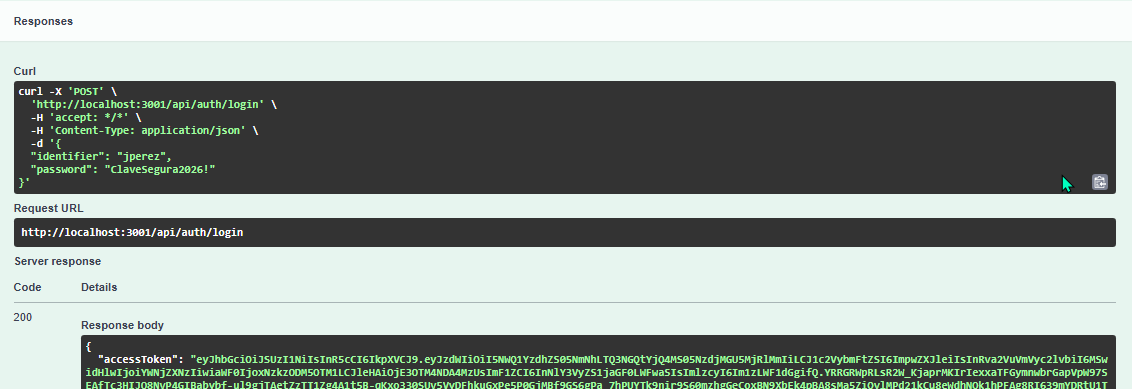
\includegraphics[width=0.8\textwidth]{cap (2).png}
    \caption{Acceso válido al sistema usando las credenciales de ADMIN}
    \label{fig1}
\end{figure}

\begin{figure}[H]
    \centering
    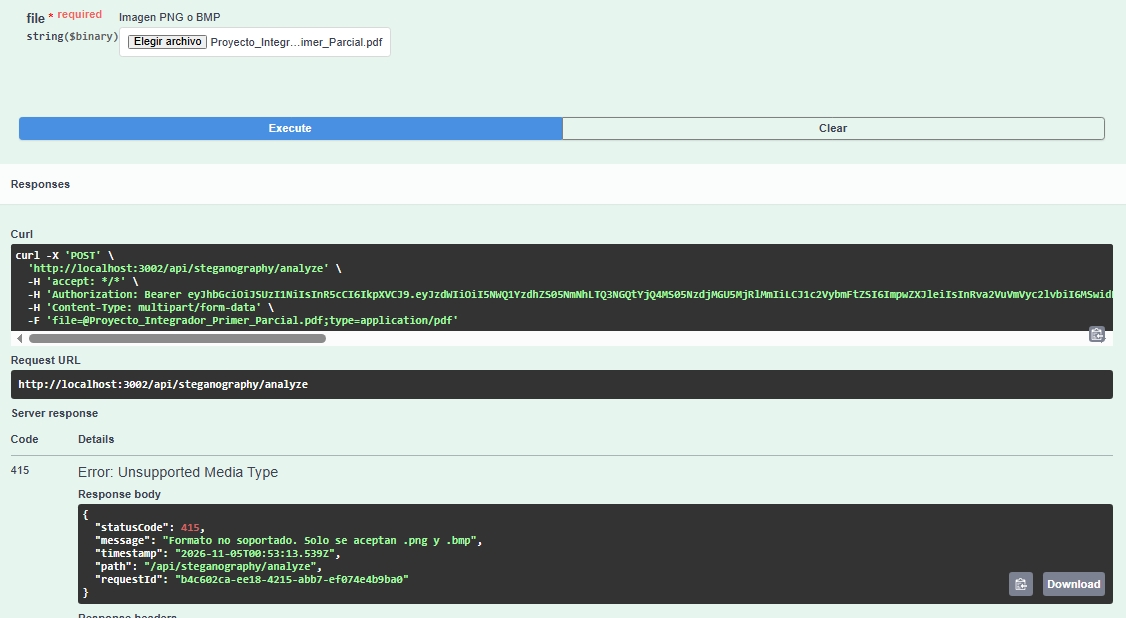
\includegraphics[width=0.8\textwidth]{cap (1).jpeg}
    \caption{Validación de esteganografía de un archivo PDF (Rechaza el archivo)}
    \label{fig1}
\end{figure}

\begin{figure}[H]
    \centering
    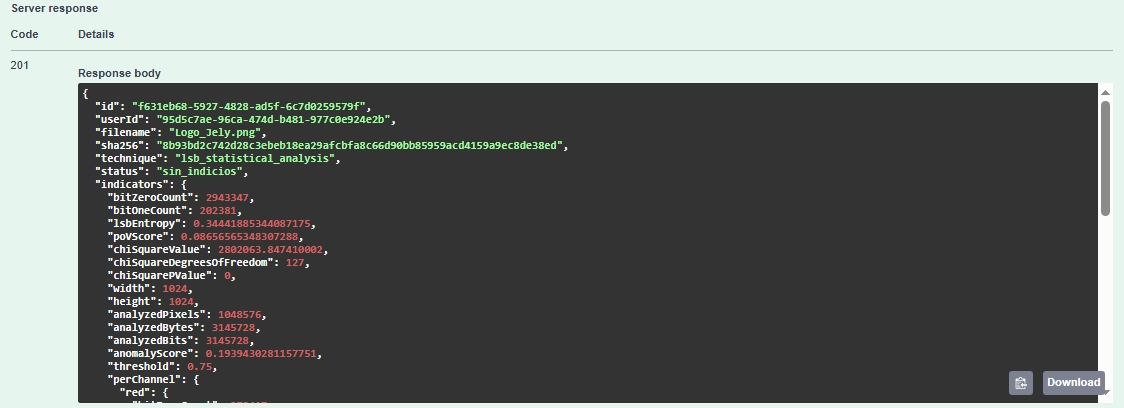
\includegraphics[width=0.8\textwidth]{cap (5).jpeg}
    \caption{Aceptación de un archivo permitido (png)}
    \label{fig1}
\end{figure}

\begin{figure}[H]
    \centering
    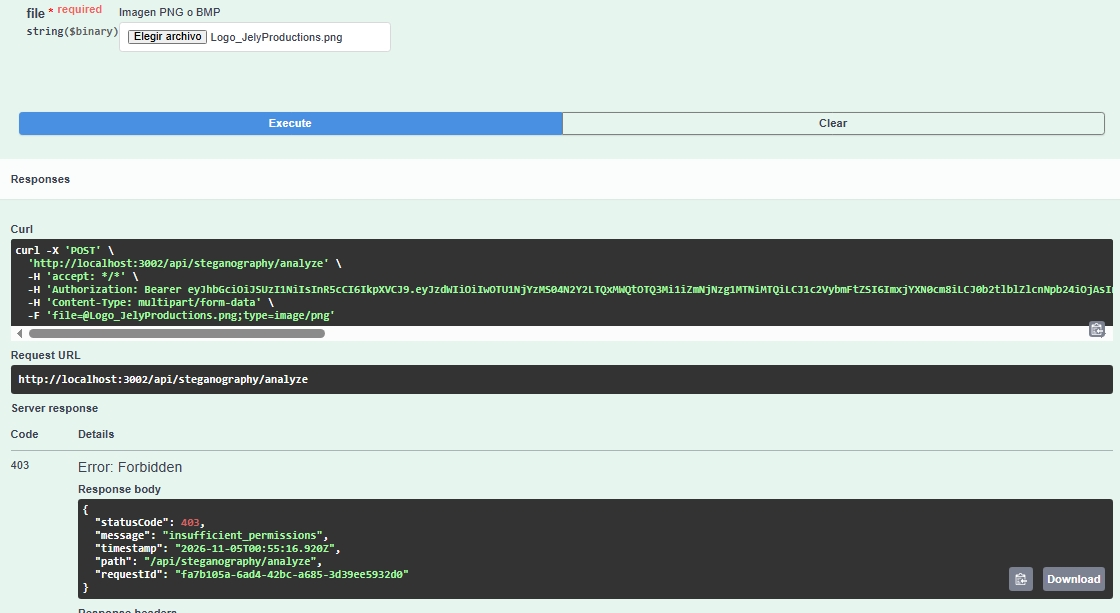
\includegraphics[width=0.8\textwidth]{cap (4).jpeg}
    \caption{Intento de analizar esteganografía desde rol usuario (Insuficientes permisos)}
    \label{fig1}
\end{figure}



% ============================================================
\subsection{Estructura del entregable}
% ============================================================

\begin{lstlisting}[caption={Organización del proyecto.}]
secure-chat-proyecto-DJF/
  docker-compose.yml       Orquestacion de auth-db, auth-migrate, auth,
                           stego-db, stego-migrate y stego
  .env.example             Plantilla de variables de entorno
  README.md                Guia de operacion y pruebas
  ms-auth-nestjs/          Servicio AUTH (NestJS), migraciones, seed,
                           pruebas unitarias y e2e, claves locales
  ms-stego-nestjs/         Servicio STEGO (NestJS), detector LSB,
                           validacion, migraciones y pruebas unitarias
  Informe/                 Este informe en LaTeX y PDF
\end{lstlisting}

\subsection{Resumen de contratos OpenAPI}

AUTH expone su contrato Swagger en \url{http://localhost:3001/docs} y STEGO en
\url{http://localhost:3002/docs} cuando \code{SWAGGER_ENABLED=true}. Los contratos
documentan esquemas de entrada, respuestas, códigos de error y seguridad Bearer.
Las rutas de negocio usan el prefijo \code{/api}; el endpoint interno de autorización
queda fuera de ese prefijo y se autentica con \code{X-Service-Key}.

\begin{resultbox}[Trazabilidad]
Los archivos de código, migraciones, pruebas y contratos están dentro del entregable
y pueden regenerarse con los comandos del capítulo de pruebas. No se incluyen
secretos reales en la documentación ni en el informe: \code{.env} y los archivos
\code{*.pem} están ignorados por Git.
\end{resultbox}


% ============================================================
\section{Conclusiones}
% ============================================================

La separación entre AUTH y STEGO permitió construir un backend con límites de
confianza explícitos. AUTH concentra identidad, claves y decisiones de autorización;
STEGO concentra la validación y el análisis de archivos. La consulta de autorización
en cada operación sensible resolvió el problema de tokens que sobreviven a un cambio
de rol, y la clave de servicio protegió el canal interno sin compartir la clave
privada RSA.

El detector LSB cumple el objetivo de triage: distingue imágenes sintéticas de
control de variantes con carga LSB, mantiene la reproducibilidad de las métricas y
rechaza archivos inválidos sin procesarlos. La combinación de entropía, igualación de
pares y chi-cuadrado es más robusta que una sola señal, aunque no sustituye una
revisión forense. La principal limitación es la tasa de falsos negativos ante
esteganografía adaptativa; el siguiente paso sería ampliar el corpus, calibrar los
umbrales con datos etiquetados y agregar análisis de dominio de transformada.

La evidencia obtenida ---83 pruebas unitarias aprobadas y una suite e2e de AUTH de 30
pruebas--- permite afirmar que la versión entregada es reproducible, operable y
coherente con los controles documentados. El proyecto deja además una base clara para
incorporar HTTPS, rotación de claves, observabilidad centralizada y despliegue en un
entorno con secretos administrados.

% ============================================================
\addcontentsline{toc}{section}{Referencias}
% ============================================================

\begin{thebibliography}{9}

\bibitem{iso27001}
ISO/IEC. \emph{ISO/IEC 27001:2022 --- Information security, cybersecurity and
privacy protection --- Information security management systems --- Requirements}.
Ginebra: ISO, 2022.

\bibitem{iso27034}
ISO/IEC. \emph{ISO/IEC 27034-1:2011 --- Application security --- Part 1: Overview
and concepts}. Ginebra: ISO, 2011.

\bibitem{owaspasvs}
OWASP Foundation. \emph{OWASP Application Security Verification Standard (ASVS)}.
Versión 4.0.3, 2021. Disponible en \url{https://owasp.org/www-project-application-security-verification-standard/}.

\bibitem{owaspupload}
OWASP Foundation. \emph{File Upload Cheat Sheet}. Disponible en
\url{https://cheatsheetseries.owasp.org/cheatsheets/File_Upload_Cheat_Sheet.html}.

\bibitem{rfc7519}
M. Jones, J. Bradley y N. Sakimura. \emph{RFC 7519: JSON Web Token (JWT)}.
IETF, 2015.

\bibitem{rfc8725}
M. Jones, J. Bradley y N. Sakimura. \emph{RFC 8725: JSON Web Token Best Current
Practices}. IETF, 2020.

\bibitem{nist800207}
S. Rose, O. Borchert, S. Mitchell y S. Connelly. \emph{NIST SP 800-207: Zero Trust
Architecture}. NIST, 2020.

\bibitem{shannon}
C. E. Shannon. \emph{A Mathematical Theory of Communication}. Bell System Technical
Journal, 27(3):379--423, 1948.

\bibitem{fridrich}
J. Fridrich, M. Goljan y R. Du. \emph{Reliable Detection of LSB Steganography in
Color and Grayscale Images}. Proceedings of the ACM Workshop on Multimedia and
Security, 2001.

\end{thebibliography}

\appendix

\end{document}
